\documentclass[12pt]{article}

\usepackage{lmodern}
\usepackage[T1]{fontenc}
\usepackage[spanish,activeacute]{babel}
\usepackage[utf8]{inputenc}
\usepackage{mathtools}
\usepackage{enumerate}
\usepackage{amsthm}
\usepackage{amssymb}
\usepackage{float}
\usepackage{subfig}
\usepackage{anysize}
\usepackage{wrapfig}

\marginsize{2cm}{2cm}{2cm}{2cm}

\title{Temas Ingeniería, Empresa y Sociedad}
\author{ }

\newtheoremstyle{definition_wo_parentheses}
  {\topsep}% measure of space to leave above the theorem. E.g.: 3pt
  {\topsep}% measure of space to leave below the theorem. E.g.: 3pt
  {}% name of font to use in the body of the theorem
  {0pt}% measure of space to indent
  {\bfseries}% name of head font
  {.}% punctuation between head and body
  { }% space after theorem head; " " = normal interword space
  {\thmname{#1}\thmnumber{ #2}\thmnote{ #3}}
  
\theoremstyle{definition_wo_parentheses}	
\newtheorem{definicion}{Definición}[section]

\begin{document}
\maketitle

\section{Tema 1: La empresa y la dirección de empresas}
\definicion{Organización}: Unidad coordinada formada por un mínimo de dos personas que trabajan para alcanzar un objetivo o conjunto de objetivos comunes.
\definicion{Empresa}: Organizaciones que proveen bienes o servicios cuya finalidad es la obtención de beneficios (diferencia entre ingresos y gastos).

\subsection{Los subsistemas funcionales de la empresa}
La empresa como sistema puede ser descompuesta en subsistemas que poseen las características del sistema general. Desde una perspectiva tradicional proponemos la división de la empresa en subsistemas funcionales de: financiación, marketing, producción, investigación, desarrollo, personal, etc.\\
\textbf{Crítica}: suponer que tales subsistemas constituyen unidades aisladas, cuando en realidad están en continua interacción.\\
\textbf{Solución}: Subsistema management (administrativo).\\

\textsc{El subsistema management} tiene diferentes funciones:
\begin{enumerate}
\item \textbf{Función general}: Integrar las distintas partes y elementos de la empresa entre sí e integrar la empresa con su entorno.
\item \textbf{Funciones específicas}: 
\begin{enumerate}
\item Planificación: Implica la definición de objetivos, conductas y acciones concretas para alcanzarlos tanto a nivel global como a nivel de los diferentes subsistemas con la finalidad de proyectar la empresa en el futuro.
\item Organización: Tiene como objetivo establecer un orden interno coherente que permita a la empresa funcionar con unidad dentro y frente a su entorno. Implica la estructuración de las relaciones interpersonales y la integración y coordinación del esfuerzo de todos los miembros a pesar de intereses divergentes.
\item Dirección: Liderar, motivar y gestionar grupos.
\item Control: Debido a la naturaleza abierta del sistema empresa, es un complemento necesario para la planificación. (Controlar que todo vaya según lo previsto).
\end{enumerate}
\end{enumerate}

\textbf{Funciones gerenciales secuenciales}.\\
La \underline{planificación} (definir metas, estableces estrategias y desarrollar subplanes para coordinar las actividades), la \underline{organización} (determinar qué debe hacerse, cómo se hará y quién deberá hacerlo), la \underline{dirección} (dirigir y motivar a los participantes y resolver conflictos) y el \underline{control} (vigilar las actividades para asegurarse de que se cumplan conforme a lo planeado), en este orden, conducen a alcanzar el propósito establecido de la organización.\\

Sin embargo el proceso administrativo tiene una \textbf{naturaleza interactiva} y todas las tareas se relacionan entre sí: en \underline{planificación}, los gerentes usan la lógica y los métodos para analizar metas y acciones; en \underline{organización}, los gerentes ordenan y asignan el trabajo, la autoridad y los recursos para alcanzar las metas de la organización; en \underline{dirección}, los gerentes dirigen, influyen y motivan a los empleados para que realicen las tareas esenciales y en \underline{control}, los gerentes se aseguran de que la organización se dirige hacia los objetivos de la organización.

\section{Tema 2: El empresario}
\definicion{Empresario}: Persona o grupo de personas (órgano colegiado) que da vida a la empresa: coordina, dirige y controla el proceso productivo.

\subsection{La dirección: Funciones y niveles}
\begin{enumerate}
\item \textbf{Diferenciación vertical}: Compuesta por una alta dirección, directivos medios y supervisores de primera línea. 
\item \textbf{Diferenciación horizontal}: Compuesta por directivos generalistas arriba y directivos generalistas y directivos funcionales por debajo de los primeros directivos generalistas.
\end{enumerate}

	Como ejemplo, si una empresa tiene varias secciones para diferentes productos, pero sólo tiene un departamento, por ejemplo, de publicidad, legal o económico común a todas las secciones, será diferenciación vertical. Por el contrario, si cada sección tiene un departamento propio para estos asuntos, será diferenciación horizontal.

\begin{figure}[H]
 \centering
  \subfloat[Diferenciación Horizontal]{
   \label{f:difH}
    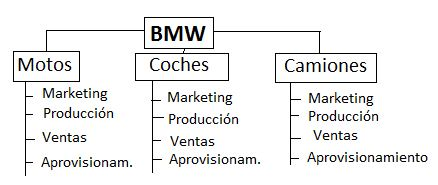
\includegraphics[width=0.5\textwidth]{difHorizontal}}
  \subfloat[Diferenciación Vertical]{
   \label{f:difV}
    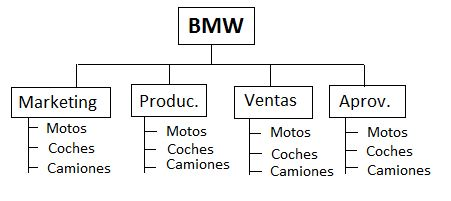
\includegraphics[width=0.5\textwidth]{difVertical}}
 \caption{Ejemplo diferenciación}
 \label{f:dif}
\end{figure}

\begin{figure}[H]
\centering
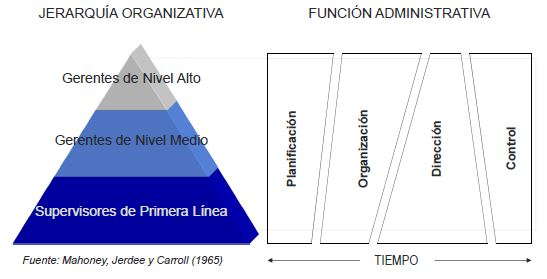
\includegraphics[width=0.65\textwidth]{jerarquia}
\caption{Las funciones y la jerarquía organizativa}
\label{fig:jerarquia}
\end{figure}

La \textbf{alta dirección} está formada por personas con responsabilidad sobre toda la empresa y de las que, en última instancia, depende su éxito o su fracaso. Sus funciones básicas pasan por fijar los grandes objetivos y estrategias que deberán alcanzarse en el largo plazo de la empresa. Aquí se incluiría el denominado comité ejecutivo de la empresa, que lo formaría el CEO junto con aquellas personas que él considere que participan en los procesos de análisis de generación de alternativas y elección de las principales decisiones de la empresa.\\

La \textbf{dirección media} está formada por los directivos de una escala inferior, entre los de primer nivel y la alta dirección. Son responsables de desarrollar las decisiones que se han tomado en el nivel superior en relación a su área de responsabilidad y en coordinación con las demás. En este sentido, establecen objetivos a medio y corto plazo, planifican y controlan las acciones para su logro, y organizan y dirigen a las personas que tienen que llevarlas a cabo. Son además el enlace jerárquico para la transmisión de las decisiones desde los niveles más altos a los más bajos.\\

La \textbf{dirección de primera línea} son los encargados del seguimiento diario de los empleados que realizan las actividades propias del objeto de la empresa. Su principal responsabilidad es garantizar que se cumplen los objetivos fijados que les vienen designados por el nivel superior.

\subsection{Caracterización de la figura del empresario}
\begin{enumerate}
\item \underline{Autoestima/Autoconfianza}: seguridad en sí mismos y creencia de que pueden desarrollar actividades con éxito.
\item \underline{Determinación para terminar tareas y tener éxito}: capacidad para concentrarse en tareas específicas para llevarlas a buen fin con garantías de éxito.
\item \underline{Persistencia}: Actitud de ``seguir intentándolo'' hasta tener éxito.
\item \underline{Voluntad y capacidad para tomar riesgos controlados}: aunque la mayor parte de los empresarios son adversos al riesgo, están dispuestos a asumir los riesgos necesarios para lograr el éxito (de una manera calculada e intentando minimizar dichos riesgos).
\item \underline{Optimismo sobre los resultados de sus acciones}: se tiene una gran confianza en que los esfuerzos darán sus resultados, lo que influye en la persistencia para seguir trabajando hasta lograr el éxito.
\item \underline{Creatividad. Capacidad de ver la necesidad y el resultado final de sus esfuerzos}: los empresarios ven las cosas ``de otra manera'', anticipando tanto las necesidades del mercado como los posibles resultados de sus acciones.
\item \underline{Enfoque. Orientación hacia objetivos}: el empresario es capaz de centrarse en objetivos y actuar para lograr los mismos.
\item \underline{Previsión/Visión de futuro}: para hacer cambios, el empresario debe prever y visualizar cómo afectarán esos cambios al futuro.
\item \underline{Tolerancia al fracaso. Falta de voluntad para aceptar el fracaso y capacidad de aprender}\\ \underline{de los errores}: los empresarios ven el fracaso como una parte más del proceso del logro del éxito, aprendiendo de sus errores y buscando soluciones satisfactorias que permitan superar los errores.
\item \underline{Responsabilidad}: los empresarios toman el control de las situaciones y aceptan la responsabilidad de los resultados alcanzados (ya sea éxito o fracaso). Los empresarios son líderes que toman la responsabilidad de seguir hacia delante.
\end{enumerate}

\section{Tema 3: Objetivos, planificación y control}
\subsection{La planificación de la empresa: concepto y tipos}
Toda empresa necesita una planificación básica para poder funcionar. La planificación empresarial marca los objetivos a alcanzar por la empresa y los medios para lograr dichos objetivos.
\definicion{Sistema de planes específicos establecidos por la dirección de la empresa que fija tanto los objetivos como las estrategias y políticas para alcanzarlos. Igualmente se puede definir como un proceso que establece cuáles son las unidades de decisión en la empresa y los métodos de elección de las diferentes acciones que ésta debe desarrollar para alcanzar los objetivos que se haya propuesto.}\\

\textbf{Requisitos a cumplir por la función de planificación}:
\begin{enumerate}
\item \underline{Cumplimiento de los objetivos}: cumplir los fines de la empresa.
\item \underline{Eficacia en la planificación}: debe procurar obtener los objetivos con las mínimas consecuencias y con beneficios que superen los costes.
\item \underline{Generalización de la planificación}: debe llegar a todos los subsistemas de la empresa y que todos conozcan cuáles son los objetivos, cómo alcanzarlos y con qué medios.
\item \underline{Eficiencia de los planes en términos de máximo rendimiento de los recursos}: alcanzar los objetivos con el menor empleo posible de recursos.
\end{enumerate}

\textbf{Tipos}:
\begin{enumerate}
\item \textbf{Según el tipo de actividad}:
\begin{enumerate}
\item \underline{Planificación general}: afecta al conjunto de actividad empresarial.
\item \underline{Planificación específica}: afecta a cada una de sus áreas de actividad específica.
\end{enumerate}
\item \textbf{Según la temporalidad}: Planificación a corto plazo/medio plazo/largo plazo.
\item \textbf{Según el futuro que planifique}:
\begin{enumerate}
\item \underline{Planificación rígida}: para un futuro cierto que permita establecer acciones definidas en el presente.
\item \underline{Planificación flexible}: para un futuro incierto que establece diferentes alternativas previendo las posibles alteraciones.
\end{enumerate}
\end{enumerate}

Según estos criterios se obtiene la siguiente clasificación:
\begin{enumerate}
\item \textbf{Planificación estratégica}: La alta dirección establece objetivos a largo plazo (más de 1 año). Es una planificación compleja que se basa en el estudio del entorno y de la propia organización, en la que intervienen gran cantidad de variables, muy amplia en contenido (ya que afecta a toda la organización) y que actúa con información externa e interna.
\item \textbf{Planificación de gestión}: La alta dirección y los directores de departamento establecen objetivos a medio y corto plazo (menos de 1 año). Es una planificación menos compleja que la anterior ya que se basa en la información interna y en los objetivos marcados por la propia planificación estratégica y su contenido es mucho más específico.
\item \textbf{Planificación operativa}: Los directores de departamento y los mandos intermedios establecen objetivos rutinarios (diarios y semanales). Es una planificación de baja complejidad que se basa en estándares técnicos y operaciones rutinarias. Para ello utiliza información interna y técnica.
\end{enumerate}

\subsection{Los objetivos de la empresa, concepto y tipología}
\definicion{\textbf{Objetivos empresariales}}: Fines hacia los cuales están dirigidas las actividades organizacionales e individuales de una empresa.\\

\textbf{Jerarquía de los objetivos}: Los objetivos se clasifican en diferentes niveles de la siguiente manera:
\begin{enumerate}
\item \textbf{Misión u objetivo supremo}: Se denomina también fin o finalidad de la empresa y constituye aquello que la empresa quiere ser, cuáles son sus aspiraciones y cuál va a ser su comportamiento. Al definir el fin de la empresa existen dos enfoques:
\begin{enumerate}
\item Hace referencia a la \underline{filosofía que adopta la empresa}, su visión de la actividad, definición de unos valores y de una política general de conducta.
\item Se refiere a la definición de la \underline{propia actividad de la empresa}: a qué se dedica la empresa, cuál es su negocio.
\end{enumerate}
\item \textbf{Objetivos generales}: Son objetivos de carácter estratégico y constituyen las metas de la empresa a largo plazo y a nivel global. Al establecer estos objetivos se analiza:
\begin{enumerate}
\item La situación del entorno (amenazas y oportunidades).
\item La situación de la empresa (fuerzas y debilidades).
\end{enumerate}
\item \textbf{Subobjetivos o metas (objetivos operacionales)}: Se fijan en todas y cada una de las unidades de la empresa a fin de concretar los objetivos generales y hacerlos operativos. Estos objetivos son a corto plazo y se asignan específicamente a unidades o personas de la organización.
\item \textbf{Acciones}: Representan el último nivel de concreción. Son un conjunto de reglas, pautas, procedimientos y recomendaciones realizadas para que la base operativa de la empresa cumpla con los objetivos establecidos.
\end{enumerate}

Los objetivos generales y los subobjetivos operacionales constituyen el sistema de objetivos de la empresa.\\
Normalmente en las empresas aparecen conflictos entre los diferentes objetivos y subobjetivos. Será la dirección de la empresa la encargada de jerarquizarlos, ordenarlos y compatibilizarlos. De esta manera se puede distinguir entre:
\begin{enumerate}
\item \textbf{Objetivos individuales}: Son aquellos que pretenden alcanzar las personas o grupos componentes de la organización. Se pueden distinguir diferentes grupos dentro de la empresa con sus correspondientes objetivos:
\begin{enumerate}
\item \underline{Propietarios del capital}: Maximizar su inversión. Con ánimo de control (a largo plazo) o simples inversionistas (a corto plazo).
\item \underline{Empleados}: Maximizar su remuneración, seguridad en el empleo y la promoción profesional.
\item \underline{Directivos}: Maximizar el crecimiento de la empresa como medio de desarrollo y prestigio profesional.
\end{enumerate}
\item \textbf{Objetivos del sistema}: Aquellos que responden a la visión de la empresa. Son iguales para todas las empresas por su generalidad:
\begin{enumerate}
\item \underline{Objetivo de eficiencia}: Obtener la máxima producción y beneficio bajo los criterios de economicidad y rentabilidad.
\item \underline{Objetivos de crecimiento}: Procurar el crecimiento armónico de la empresa y de todas sus unidades.
\item \underline{Objetivo de control}: Regular la actividad económica de la empresa manteniendo un control interno (empresa) y externo (poder de mercado).
\item \underline{Objetivo de supervivencia}: Voluntad de seguir operando.
\end{enumerate}
\end{enumerate}

\subsection{El control en la empresa}
El proceso de control es un proceso dirigido a verificar si los resultados obtenidos se ajustan a los resultados planificados.\\

\textbf{Pasos en el proceso de control}:
\begin{enumerate}
\item \underline{Determinar los puntos críticos de control}: Son factores que pueden indicar, de manera eficiente, si se está realizando bien un plan o no.
\item \underline{Establecer normas o estándares de control}: Una norma o estándar es una referencia para considerar los resultados que se deben ir alcanzando. Son medidas para evaluar los planes. Es la traducción numérica de los objetivos, para poder establecer comparaciones.
\item \underline{Medición del desempeño}: Analizar si los resultados obtenidos  se ajustan a los estándares establecidos anteriormente.
\item \underline{Tomar medidas correctivas}: Corregir las desviaciones para poder conseguir los objetivos. Hay que corregir la causa de la desviación (no el síntoma).
\end{enumerate}


\section{Tema 4: Organización}

\subsection{Introducción a la función de organización}

\begin{definicion}[Organización] 
	Diseño del armazón material y humano que actuará de soporte para la ejecución de los planes establecidos.
\end{definicion}

\begin{itemize}
\item El punto de partida es el conocimiento de la misión, así como de los objetivos (estratégicos y operativos).

\item Utilización de diferentes herramientas (parámetros de diseños para construir la estructura. Implica tomar decisiones internas sobre: 

	\begin{itemize}
		\item Diseño de puestos de trabajo (especialización, formalización y preparación).
		\item Agrupación de puestos en unidades (departamentalización)
		\item Tamaño de las unidades.
		\item Establecimiento de vínculos laterales para coordinar departamentos.
		\item Descentralización de la toma de decisiones.
	\end{itemize}
	
\item Consideración de la incidencia de los factores de contingencia en los parámetros del diseño. Son factores de contingencia la edad y el tamaño de la empresa, el sistema técnico y el entorno
\end{itemize}

\subsection{Diseño organizativo}

\subsubsection{Mecanismos de coordinación}

\paragraph{Adaptación mutua.} Consigue la coordinación del trabajo mediante la simple comunicación informal. El control corre a cargo de quienes lo realizan. Asumible cuando los grupos son pequeños.

\paragraph{Supervisión directa.} Una persona es responsable del trabajo de los demás. Más frecuente conforme los grupos crecen.

\paragraph{Normalización.} Coordinación incorporada en el programa de trabajo. Menor necesidad de una comunicación continua. Son mecanismos adquiridos, facilita el crecimiento de los grupos. 

\subsubsection{Partes de la organización}

Entre las partes de la organización se distinguen las unidades de líneas; trabajan en la empresa, en el servicio que presta la empresa; y las unidades de \textit{staff}, que no trabajan para el objetivo de la empresa, sino que ofrecen servicios necesarios para ésta, de apoyo a la organización, no participan en la producción.

Las unidades de línea son:
\paragraph{Núcleo de operaciones.} Obreros. Miembros de la organización que realizan el trabajo básico directamente relacionado con la producción de bienes y servicios. Sus funciones son asegurar la entrada del material para la producción, su transformación, distribución de la mercancía. Constituyen el centro de toda organización. Es donde la normalización se aplica con mayor profundidad.

\paragraph{Ápice estratégico.} Es el órgano que se ocupa de que la organización cumpla, efectivamente, con su misión y que satisfaga convenientemente los intereses de los grupos y personas involucradas en la misma (socios, Estado, sindicatos, etc.)\\
Sus funciones son supervisar la organización y velar por que funcione debidamente como una unidad integrada, mantener relaciones con el entorno y desarrollar las estrategias de la organización. Desempeña un papel vital en la formulación de la estrategia. Su trabajo se caracteriza por un mínimo de repetición y normalización. La adaptación mutua es el mecanismo habitual.

\paragraph{Línea media.} Abarca desde los mandos situados bajo el ápice estratégico hasta los supervisores de primera línea (los que ejercen la supervisión directa sobre los operarios). Sus funciones son enlazar el ápice estratégico con el núcleo de operaciones, transmitiendo y ejecutando decisiones e información.

Las unidades de \textit{staff} se dividen en:

\paragraph{Tecnoestructura o analistas.} Formada por los analistas (y su personal administrativo) que sirven a la organización operando sobre el trabajo de los demás miembros de la misma. No intervienen directamente en el flujo de operaciones, aunque lo diseñan, planifican, cambian y preparan a las personas que lo realizan.

\paragraph{\textit{Staff} de apoyo.} Unidades especializadas cuya función consiste en proporcionar asistencia a la organización fuera del flujo de trabajo de operaciones corrientes. Estos servicios se pueden subcontratar o ser gestionados por la organización, controlándolos directamente. Estas unidades pueden funcionar como miniorganizaciones, con su propio núcleo de operaciones, línea media y ápice estratégico. Son ejemplos de \textit{staff} de apoyo servicios como el de cafetería o limpieza de una empresa que se dedique a otro sector.

	El componente administrativo de la organización está compuesto por el ápice estratégico, la línea media y la tecnoestructura. 
	
	
\subsection{Dimensiones del diseño organizativo}

\subsubsection{Diseño de puestos}

\begin{definicion}[Diseño de puestos]
Es el proceso mediante el cual se enseñan las habilidades y conocimientos relacionados con el puesto. 
\end{definicion}

	Existen dos tipos de puestos de trabajo:
	
\begin{enumerate}
\item No cualificado. Al realizarse un trabajo sumamente racionalizado, supone una extensa especialización tanto horizontal como vertical, siendo a menudo controlado y coordinado por la formalización directa.

\item Profesional. Corresponde a un trabajo que no puede especializarse fácilmente en la dimensión vertical ni ser formalizado por la tecnoestructura de la organización, teniendo una especialización horizontal y consiguiéndose a menudo una coordinación mediante la normalización de habilidades en exhaustivos programas de preparación, que suelen impartirse fuera de la organización.
\end{enumerate}

\paragraph{Formalización del comportamiento} La formalización del comportamiento representa la forma en la que la organización limita la libertad de acción. Mediante este parámetro se normalizan los procesos de trabajo. La formalización se refiere a la existencia de descripciones explícitas o implícitas relativas a reglas, procedimientos y procesos de toma de decisiones, de comunicación de instrucciones y de transmisión de información que indican en todo momento lo que ha de hacer el trabajador.\\
La formalización la realizan los analistas del \textit{staff}, lo que implica para los trabajadores una pérdida de control de sus actividades, dando lugar a una especialización vertical del puesto. La formalización del trabajo es mayor en los niveles operativos, ya que en estos se realizan las actividades más sencillas y repetitivas (especialización horizontal). Las organizaciones que se basan ante todo en la formalización del comportamiento para conseguir una coordinación suelen denominarse burocracias.

\begin{enumerate}
\item Formas burocráticas. Basada en la formalización del comportamiento. Son organizaciones con circunstancias estables. Basada en la normalización
\item Formas orgánicas. Relaciones de trabajo abiertas e informales. Organizaciones que necesitan innovaciones. Basada en la adaptación mutua.
\end{enumerate}

Definiremos la estructura orgánica como la ausencia de normalización. 

\begin{definicion}[Especialización del trabajo] 
	La especialización es la destreza que consigue un individuo para la realización de unas tareas.
\end{definicion}

Los trabajos sumamente repetitivos se tienden a dividir cada vez más en tareas más sencillas para que el trabajador las aprenda antes y las realice de forma más rápida. La especialización se realiza en dos aspectos:

\begin{enumerate}[a]
\item Especialización horizontal. Realización de pocas tareas o con poco contenido.
\item Especialización vertical. Existe poco control sobre el trabajo. La especialización vertical del puesto separa la realización del trabajo y la administración del mismo
\end{enumerate}

Lo contrario de la especialización del puesto es la ampliación.

\subsubsection{Diseño de la superestructura}

El siguiente paso es agrupar los puestos de trabajo que hemos diseñado en unidades, y diseñar el tamaño de cada unidad. Esto da los parámetros de diseño \underline{agrupación de unidades} y \underline{tamaño de la unidad}.


\begin{description}
\item [Agrupación de unidades] Las bases de agrupación son: Por conocimientos y habilidades, según el proceso de trabajo y la función, según el \textit{output}, por clientes o por zonas geográficas. Siguiendo la clasificación de Mintzberg, las dos primeras son agrupaciones funcionales y las restantes agrupaciones según el mercado.

\item [Tamaño de la unidad] El tamaño de la unidad es determinado por el concepto de ámbito o tramo de control
\end{description}


\begin{definicion}[Ámbito o tramo de control] Número de subordinados que un gerente puede supervisar de manera eficaz. Este concepto determina el número de niveles y gerentes de una organización.
\end{definicion}

\begin{description}
\item [Estructuras altas] pequeñas unidades y tramos de control estrechos.
\item [Estructuras planas] grandes unidades y tramos de control amplios.
\end{description}


\subsubsection{Diseño del sistema decisor}

\begin{definicion}[Centralización] 

	Describe dónde está la autoridad para la toma de decisiones.
	
\end{definicion}

	Pese a que la centralización coordina la toma de decisiones, la descentralización tiene como ventajas el reparto de la responsabilidad, la rapidez en la toma y constituye un estímulo a la motivación.
	
\subsection{Los factores de contigencia}

\paragraph{Edad y tamaño} Cuanto más antigua y mayor, habrá una mayor formalización y la estructura será más compleja.

\paragraph{Sistema técnico} Cuanto más regulador sea el sistema técnico, habrá mayor formalización. Cuanto más sofisticado, habrá una mayor descentralización selectiva.

\paragraph{El entorno} Cuanto más dinámico, más orgánica resulta la estructura. Cuanto más complejo, más descentralizada. Disparidades en el entorno estimulan la descentralización.

\subsection{Configuraciones estructurales}

\begin{definicion}[Eficacia]
Congruencia interna de las variables de diseño. Congruencia de dichas variables con los factores de contingencia.
\end{definicion}

Las configuraciones estructurales se diferencian por el mecanismo de coordinación predominante y por el grado de centralización:

\begin{enumerate}[I]
\item Estructuras orgánicas $\rightarrow$ Ausencia de normalización.
\begin{enumerate}[a]
\item Estructuras orgánicas centralizadas: \underline{Estructuras simples}
\item Estructuras orgánicas descentralizadas: \underline{Adhocracias}
\end{enumerate}
\item Estructuras burocráticas $\rightarrow$ Normalización.
\begin{enumerate}[a]
\item Estructuras burocráticas centralizadas: \underline{B. maquinales}
\item Estructuras burocráticas descentralizadas: \underline{B. profesionales}
\end{enumerate}
\end{enumerate}


\begin{description}
\item[Estructura simple] Se caracteriza por la falta de elaboración. Dispone de una tecnoestructura mínima o nula, reducido \textit{staff} de apoyo, división poco estricta del trabajo, diferenciación mínima entre unidades y una pequeña jerarquía directiva. Presenta poco comportamiento formalizado. Es principalmente orgánica. Coordinación mediante supervisión directa. La estructura consiste a menudo en un ápice estratégico de una sola persona y un núcleo de operaciones orgánico.
\item[Burocracia maquinal] Se caracteriza por tareas de operaciones altamente especializadas y rutinarias, procedimientos sumamente formalizados en el núcleo de operaciones, una proliferación de reglas, normas y comunicación formal a través de toda organización, unidades de gran tamaño en el núcleo de operaciones, tareas agrupadas a base de su función, poder de decisión relativamente centralizado, elaborada estructura administrativa con una clara distinción entre línea y \textit{staff}. La burocracia maquinal genera sus normas y recurre a la autoridad de naturaleza jerárquica.

\item[Burocracia profesional] Cuenta para su coordinación con la normalización de las habilidades y su correspondiente parámetro de diseño, la preparación. Contrata a especialistas debidamente preparados para su núcleo de operaciones, confiriéndoles a continuación un control considerable sobre su propio trabajo. Estructura sumamente descentralizada. El núcleo de operaciones constituye la parte central. Tecnoestrucura y línea media no muy elaboradas. Las normes surgen, por regla general, fuera de su propia estructura. Hace hincapié en la autoridad de naturaleza profesional.

\item[Adhocracia] Nionguna de las estructuras anteriores son capaces de realizar una innovación sofisticada. La estructura simple innova pero de forma sencilla. Las burocracias son estructuras de rendimiento y no de solución de problemas. Es orgánica, tiene escasa formalización. Elevada especialización horizontal del puesto basada en la preparación. Tendencia a agrupar a los especialistas en unidades funcionales en lo correspondiente a asuntos internos. Uso de los dispositivos de enlace para fomentar la adaptación mutua y una descentralización selectiva.

\item[Burocracia divisionalizada] Se trata de una serie de entidades semiautónomas acopladas mediante una estructura administrativa central. Estas entidades se denominan divisiones. La administración que las reúne se denomina sede central. El ámbito de control del ápice estratégico puede ser bastante amplio. La sede central permite a las divisiones autonomía casi completa para tomar sus propias divisiones, controlando posteriormente los resultados. Mecanismos de coordinación:Normalización de \textit{output}. Las divisiones adoptan estructuras de burocracia maquinal.
\end{description}


\section{Tema 6: El análisis del entorno}

\begin{definicion}[Entorno] 
	Sistema que va a rodear a la organización, pudiendo influir sobre ella. Conjunto de todos los elementos externos a la organización que influyen o modifican su actuación. Entorno es todo aquello que es ajeno a la organización.
\end{definicion}

	El análisis general se corresponde con la industria, el análisis específico con el sector y el análisis interno con la empresa.
	
\paragraph{Etapas del análisis del entorno}
\begin{enumerate}
\item Valorar la naturaleza del entorno $\rightarrow$ Tipología del entorno.
\item Análisis del entorno general $\rightarrow$ Análisis PESTEL
\item Análisis del entorno específico: 5 fuerzas competitivas $\rightarrow$ Competidores potenciales, rivalidad entre competidores, productos sustitutos, poder de negociación de clientes y proveedores.
\end{enumerate}

\subsection{Tipología  o naturaleza del entorno}

\begin{definicion}[Dinamismo]
El dinamismo del entorno es su grado de predecibilidad.
\end{definicion}

\begin{description}
\item[Entorno dinámico] Existen cambios y son impredecible. A más cambios, más rápidos e impredecibles, más dinámico será el entorno. Ejemplo: Sector informático.
\item[Entorno estable] No se producen cambios en los factores que influyen a la empresa o se pueden predecir con facilidad. Ejemplo: Sector comercio minorista.
\end{description}

\begin{definicion}[Complejidad]
La complejidad del entorno depende de la necesidad de conocimientos que necesita la empresa.
\end{definicion}

\begin{description}
\item[Entorno complejo]Si la organización necesita conocimientos sofisticados sobre los productos, clientes o factores. Ejemplo: Sector aeronáutico.
\item[Entorno sencillo] Cuando dicho conocimiento puede racionalizarse o se hace más comprensible. Ejemplo: Sector agrario.
\end{description}



\begin{definicion}[Diversidad]
La diversidad del entorno depende del número de variables
\end{definicion}

\begin{description}
\item[Entorno diverso] Existencia de un gran número de clientes, productos, servicios o zonas geográficas que abastecer. Ejemplo: El Corte Inglés.
\item[Entorno integrado] Si las variables que lo constituyen son reducidas y similares. Ejemplo: Autoescuelas.
\end{description}



\begin{definicion}[Hostilidad]
La hostilidad del entorno depende de la agresividad de los grupos de interés.
\end{definicion}

\begin{definicion}[Stakeholders, grupos de interés]
Grupos de personas con intereses en la empresa: propietarios, clientes, accionistas, trabajadores, proveedores...
\end{definicion}

\begin{description}
\item[Entorno hostil] Se define por la competencia, las relaciones con los sindicatos, gobiernos y grupos externos y por la disponibilidad de recursos. Ejemplo: compañías telefónicas.
\item[Entorno munificente] A menor competencia y mayor disponibilidad de recursos, el entorno es menos hostil. Ejemplo: ONCE, concesionarias de agua.
\end{description}

\subsection{Análisis del entorno general}

El objetivo es identificar los factores que influyen en el sector en el que se encuentra la organización, qué factores del entorno afectan al sector de la organización y cuáles son los más importantes en ese momento y en los próximos años.

\paragraph{Político-legal} Integra los factores administrativos, legales y reguladores dentro de los cuales la empresa debe operar. Muchos de estos factores son restrictivos para la empresa (salarios mínimos, impuestos); sin embargo otros son favorables (subvenciones, ayudas públicas, protección legal, ...)

\paragraph{Económico} Aspectos o indicadores de naturaleza económica que afectan al sistema económico donde se desenvuelve la empresa.

\paragraph{Sociocultural} Recogen tanto creencias, valores, actitudes y formas de vida de las personas que rodean a la empresa como las condiciones culturales, ecológicas, demográficas, religiosas, educativas del sistema social en su conjunto.

\paragraph{Tecnológica} El marco científico y tecnológico que caracteriza la situación de un sistema.

\subsubsection{Análisis PESTEL}

El análisis PESTEL ayuda al análisis estratégico de las siguientes formas: 

\begin{itemize}
\item Puede considerarse como lista de verificación para realizar el análisis de los distintos factores.
\item Puede ser útil para identificar una serie de generadores claves de cambio del entorno (fuerzas motrices que influirán sobre la estructura de una industria o mercado)
\item Puede ayudar a examinar las consecuencias diferenciales de las influencias externas sobre las organizaciones, ya sea históricamente o respecto al posible impacto futuro.
\end{itemize}

\begin{description}
\item[Político-legales] Legislación sobre monopolios, legislación medioambiental, política impositiva, regulación del comercio exterior, normativa laboral, estabilidad política,...
\item[Económicos] Ciclo económico, tendencia del PNB, tipos de interés, inflación, desempleo, renta disponible, disponibilidad y coste de la energía,...
\item[Socioculturales] Demografía, distribución de la renta, movilidad social, cambios en el estilo de vida, actitudes respecto a la vida y el ocio, nivel educativo, consumismo,...
\item[Tecnológicos] Gasto estatal en I+D, relación empresas-centros I+D, tasas de obscolescencia, nuevos descubrimientos, transferencia de conocimientos...
\end{description}

El test PEST puede ser extendido con -EL (Ecológico-Legal)

\subsection{Análisis del entorno específico}

\begin{definicion}[Entorno específico]
	Conjunto de circunstancias que afectan de manera concreta a un grupo determinado de organizaciones
\end{definicion}

\begin{definicion}[Sector]
	Conjunto de organizaciones que realizan la misma actividad principal.\\
	Conjunto de organizaciones que producen productos que son sustitutivos cercanos entre sí - \textit{Michael Porter}
\end{definicion}

El análisis del entorno específico se hace a través del análisis de las fuerzas competitivas, el cual consta de cinco puntos.

\subsubsection{Grado de rivalidad entre competidores existentes}

\begin{itemize}
\item Número de competidores y grado de concentración
\item Crecimiento del sector
\item Costes fijos o de almacenamiento elevado 
\item Diferenciación o costes cambiantes
\item Barreras de salida (Costes a asumir si se abandona)
	\begin{itemize}
	\item Activos especializados
	\item Costes fijos de salida
	\item Barreras emocionales
	\item Restricciones sociales y gubernamentales
	\end{itemize}
\item Intereses estratégicos: Interés en mantener un negocio porque sirve de apoyo a un negocio de mayor importancia.

\end{itemize}

\subsubsection{Competidores potenciales}

\paragraph{Barreras de entrada}
\begin{itemize}
\item Economías de escala: Reducción en los costes unitarios de fabricación por producto conforme aumenta el volumen absoluto.
\item Diferenciación del producto y costes cambiantes.
\item Necesidades o requisitos de capital
\item Acceso a los canales de distribución.
\item Desventajas en costes independientes del tamaño: Tecnología de producto patentada, acceso favorable en materias primas, ubicaciones favorables.
\item Curva de aprendizaje o efecto experiencia. 
\item Política gubernamental.
\end{itemize}

\paragraph{Reacción esperada de las organizaciones existentes en el sector} Recursos de las organizaciones existentes, experiencia histórica, compromiso con el sector

\paragraph{Potencial de beneficios del sector} Tasa de crecimiento del sector, número de competidores, concentración de las ventas.

\subsubsection{Productos sustitutos}

\begin{definicion}[Productos sustitutos]
Son productos que satisfacen las mismas necesidades que las que satisface el producto que ofrece la industria.
\end{definicion}

\paragraph{Formas de sustitución} Las formas de sustitución son mediante un producto con la misma función o ampliada, por productos reciclados o por no usar nada.

\paragraph{Determinantes de la amenaza de sustitución} Son la relación valor/precio, el coste de cambio bajo y la propensión al cambio por parte de los consumidores.

\subsubsection{Fuerza de negocio de los clientes}

Los clientes pueden amenazar con forzar la bajada de precios, exigir una calidad superior, exigir mejores servicios, y exigir mejores condiciones financieras. Esto se puede deber a que haya un alto volumen de compra, poca diferenciación de los productos suministrados, la integración hacia atrás de uniones de clientes, la rentabilidad baja, el bajo coste de cambiar de proveedor... Frente a estas tácticas de los clientes las organizaciones optan por diversificar la clientela.

\subsubsection{Poder negociador de los proveedores}

Los clientes pueden amenazar con subir los precios, bajar la calidad, variar las condiciones del servicio o la negociación colectiva mediante acuerdos o uniones entre ellos si el sector está mue fraccionado. Otras medidas son que no hayan productos sustitutivos, la importancia relativa del producto, la integración hacia adelante, el número de proveedores, o los costes de cambio.

\end{document}